%=====================================================================
%  Proyecto final, Procesamiento de Lenguaje Natural, UTEC 2026
%  Auditor ReAct: sistema multiagente con guardrails frente a Naive RAG
%=====================================================================
\documentclass[10pt,a4paper,twocolumn]{article}

\usepackage{lmodern}
\usepackage[T1]{fontenc}
\usepackage[utf8]{inputenc}
\usepackage[spanish,es-noquoting,es-tabla,es-nodecimaldot]{babel}
\usepackage{amsmath,amssymb}
\usepackage{booktabs}
\usepackage{graphicx}
\usepackage{xcolor}
\usepackage[margin=1.8cm,columnsep=0.6cm]{geometry}
\usepackage{enumitem}
\usepackage{caption}
\usepackage{microtype}
\usepackage[colorlinks=true,linkcolor=tinta,citecolor=tinta,urlcolor=tinta]{hyperref}

\definecolor{tinta}{HTML}{22303C}
\captionsetup{font=small, labelfont=bf}
\setlist{itemsep=1pt, topsep=2pt, leftmargin=*}
\hyphenpenalty=10000
\exhyphenpenalty=10000
\emergencystretch=2em
\graphicspath{{../figures/}}

\title{\textbf{Auditor ReAct: un sistema multiagente con guardrails para auditoría de hechos, razonamiento matemático y código}}
\author{Ricardo A. Acuña-Villogas \and Juan Aquino-Espinoza \and Josué Velo\\[1mm] \small Procesamiento de Lenguaje Natural, UTEC}
\date{Noviembre 2026}

\begin{document}
\twocolumn[
\maketitle
\vspace{-8mm}
\begin{center}
\begin{minipage}{0.9\textwidth}
\small
\textbf{Resumen.} Se presenta un sistema de tres agentes (Investigador, Auditor de Hechos y Redactor) coordinados con LangGraph sobre un orquestador local Qwen2.5 7B en 4 bits, con un índice FAISS de WikiQA, GSM8K y MBPP, búsqueda web y ejecución de Python. En 50 consultas de los tres datasets el sistema empata con un Naive RAG en acierto global y es algo menos fiel según RAGAS, porque esas preguntas se resuelven con una sola recuperación; supera al Naive RAG en código, donde ejecuta y verifica los tests. En 15 consultas multisalto que exigen dos documentos y un cálculo casi duplica su acierto. El Auditor mejora el resultado solo cuando su retroalimentación es accionable, y con un orquestador de 1.5B la arquitectura empeora. Para producción se propone enrutar: un paso por defecto y el grafo completo para consultas compuestas.
\end{minipage}
\end{center}
\vspace{4mm}
]

%=====================================================================
\section{Introducción}
%=====================================================================
Un Naive RAG recupera una vez y genera una vez: si el contexto recuperado no contiene la respuesta, si la pregunta exige varios pasos de cálculo o si la salida es código que debe ejecutarse, el modelo completa los huecos con texto plausible. El paradigma ReAct \cite{yao2023react} intercala razonamiento y acciones sobre herramientas, y los grafos de agentes permiten separar quién investiga de quién verifica. Este trabajo construye un sistema de tres agentes con LangGraph, un orquestador local de 7B cuantizado en 4 bits y un Auditor que puede devolver el flujo cuando detecta datos sin respaldo, y lo compara contra un Naive RAG en 50 consultas de WikiQA \cite{yang2015wikiqa}, GSM8K \cite{cobbe2021gsm8k} y MBPP \cite{austin2021mbpp}.

%=====================================================================
\section{Sistema}
%=====================================================================
\begin{figure}[t]
\centering
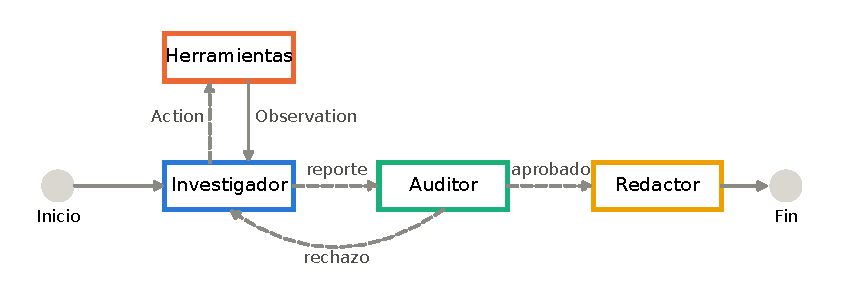
\includegraphics[width=\columnwidth]{fig1_grafo_agentes.pdf}
\caption{Grafo de control compilado en LangGraph. Las aristas punteadas son condicionales: el bucle Action y Observation entre Investigador y Herramientas, y el rechazo del Auditor que devuelve el flujo al Investigador.}
\label{fig:grafo}
\end{figure}

\textbf{Orquestador.} Qwen2.5 7B Instruct \cite{qwen2025} cuantizado en NF4 con doble cuantización \cite{dettmers2023qlora}, unos 6 GB de VRAM, con decodificación voraz. Los tres agentes comparten el modelo y difieren en su prompt de sistema.

\textbf{Agentes} (Figura~\ref{fig:grafo}).
\begin{enumerate}
\item \textbf{Investigador.} Emite un paso por turno con el formato Thought, Action, Action Input; la generación se corta en la cadena Observation y el nodo de herramientas inyecta la observación real. Tiene un máximo de 6 acciones por intento.
\item \textbf{Auditor de Hechos.} Combina dos guardrails. El determinista rechaza un reporte sin evidencia o con código que no pasa los tests del enunciado. El semántico pide al LLM contrastar el reporte con las observaciones y responder APROBADO o RECHAZADO con un motivo. Un rechazo devuelve el estado al Investigador con el motivo, hasta 2 veces.
\item \textbf{Redactor.} Convierte el reporte aprobado en la respuesta final, citando los identificadores de las fuentes.
\end{enumerate}

\textbf{Herramientas.} buscar\_kb consulta un índice FAISS de producto interno sobre embeddings normalizados de all MiniLM L6 \cite{reimers2019sbert} (similitud coseno) con 10\,758 documentos: un documento por título de WikiQA, los problemas resueltos de GSM8K train y los programas de MBPP train. buscar\_web usa DuckDuckGo con respaldo en la API de Wikipedia. ejecutar\_python corre el código en un proceso aislado con límite de 10 segundos. Cualquier error de una herramienta (un nombre inexistente, código que no imprime, un timeout o la web caída) vuelve al Investigador como Observation y no interrumpe el grafo.

\textbf{Procesamiento de datos.} WikiQA llega como pares de pregunta y oración candidata; las oraciones se agrupan por título, sin duplicados y en su orden, y cada artículo es un documento (2\,811, mediana de 1\,065 caracteres). De GSM8K se indexan los 7\,473 problemas de train con su solución (mediana 511) y de MBPP los 474 enunciados con su función de train, validation y prompt (mediana 240); los tests y el código de setup se guardan aparte para el Auditor. Los documentos son cortos y se indexan enteros, sin trocear. La respuesta oro de GSM8K es el número tras \#\#\#\#, sin comas. Para la aplicación web los mismos vectores se exportan cuantizados a int8.

\textbf{Referencia.} El Naive RAG recupera los 4 documentos más similares a la pregunta y genera la respuesta en una sola llamada, con el mismo modelo.

\begin{table*}[t]
\centering
\caption{Comparación sobre las 50 consultas. Faithfulness y Answer Relevance según el juez; acierto por tarea y global; costo por consulta.}
\label{tab:principal}
\small
\begin{tabular}{lcccccccc}
\toprule
Sistema & Faithfulness & Answer Rel. & WikiQA & GSM8K & MBPP & Acierto global & Segundos & Llamadas \\
\midrule
Multiagente 7B & 0.84 & 0.68 & 0.80 & 1.00 & 0.53 & \textbf{0.78} & 44.6 & 6.2 \\
Naive RAG 7B & 0.91 & 0.72 & 0.85 & 1.00 & 0.47 & \textbf{0.78} & 4.8 & 1.0 \\
Multiagente sin Auditor 7B & 0.84 & 0.68 & 0.80 & 0.93 & 0.47 & \textbf{0.74} & 38.6 & 4.2 \\
Multiagente 1.5B & 0.47 & 0.44 & 0.65 & 0.60 & 0.13 & \textbf{0.48} & 49.4 & 6.8 \\
Naive RAG 1.5B & 0.78 & 0.64 & 0.60 & 0.73 & 0.13 & \textbf{0.50} & 3.8 & 1.0 \\
\bottomrule

\end{tabular}
\end{table*}

%=====================================================================
\section{Diseño experimental}
%=====================================================================
Se toman con semilla fija 20 preguntas de WikiQA test con respuesta, 15 problemas de GSM8K test y 15 tareas de MBPP test (con sus tres tests en el enunciado); ninguna de las dos últimas está en el índice.

\textbf{Métricas RAGAS} \cite{es2023ragas}, con Phi 4 \cite{abdin2024phi4} como juez para evitar que el modelo se evalúe a sí mismo. Faithfulness es la fracción de afirmaciones atómicas de la respuesta que el juez deduce del contexto que el sistema recuperó. Answer Relevance es la similitud coseno media entre la pregunta y tres preguntas que el juez genera a partir de la respuesta:
\begin{equation}
\mathrm{AR} = \frac{1}{3}\sum_{i=1}^{3} \cos\big(e(q),\, e(\hat q_i)\big).
\end{equation}
\textbf{Métricas objetivas.} Corrección según el juez frente a la oración de referencia en WikiQA, número exacto en GSM8K y tests aprobados en MBPP; su promedio es el acierto global. También se registran segundos, llamadas al LLM y tokens por consulta.

\textbf{Ablaciones.} Multiagente sin Auditor; orquestador de 1.5B en lugar de 7B; y tres modelos de embeddings con distintos valores de k.

\textbf{Pipeline y análisis.} Cuatro scripts (preparación, generación, juez y figuras) se comunican por archivos JSONL con una línea por consulta, así que una corrida interrumpida se reanuda y todas las tablas de este informe se generan desde esos archivos. Como todos los sistemas responden las mismas consultas, las diferencias se analizan de forma pareada: prueba del signo sobre las consultas en que dos sistemas discrepan e intervalo bootstrap del 95\,\% (5\,000 remuestreos) para la diferencia de acierto.

%=====================================================================
\section{Resultados}
%=====================================================================

\textbf{Preguntas de los datasets} (Tabla~\ref{tab:principal}, Figura~\ref{fig:tareas}). Con 7B el multiagente y el Naive RAG empatan en acierto global. El Naive RAG es algo más fiel y relevante: sus respuestas son cortas y se apoyan en un único contexto, mientras que el multiagente redacta más afirmaciones a partir de varias fuentes. La razón del empate está en las preguntas: el documento correcto de WikiQA aparece entre los tres primeros recuperados en el 99\,\% de los casos (Anexo~\ref{sec:anexo}) y GSM8K lo resuelve el 7B sin ayuda. El multiagente solo gana en MBPP, donde ejecutar los tests aporta. Sin Auditor el acierto baja en GSM8K y MBPP.

\textbf{¿Son reales las diferencias?} (Tabla~\ref{tab:pares}). En las 50 consultas el multiagente y el Naive RAG discrepan en solo 8: cuatro las acierta cada uno, y el intervalo de la diferencia, de $-0.12$ a $0.10$, contiene el cero. La ventaja del Auditor (3 frente a 1) tampoco es concluyente con esta muestra. Hay dos efectos claros: la descomposición en multisalto (6 frente a 0) y el tamaño del orquestador (14 frente a 0 entre los Naive de 7B y 1.5B).

\begin{table}[t]
\centering
\caption{Comparación pareada; 7B salvo que se indique. Solo A y Solo B cuentan las consultas que acierta un sistema y no el otro.}
\label{tab:pares}
\footnotesize
\setlength{\tabcolsep}{3pt}
\begin{tabular}{lcccc}
\toprule
A frente a B & n & Solo A & Solo B & Prueba \\
\midrule
Multi, Naive & 50 & 4 & 4 & IC $[-0.12, 0.10]$ \\
Multi, Naive (multisalto) & 15 & 6 & 0 & $p = 0.03$ \\
Con Auditor, sin Auditor & 50 & 3 & 1 & $p = 0.63$ \\
Naive 7B, Naive 1.5B & 50 & 14 & 0 & $p < 0.001$ \\
Multi 1.5B, Naive 1.5B & 50 & 5 & 6 & $p = 1.00$ \\
\bottomrule
\end{tabular}
\end{table}

\textbf{¿De dónde sale la brecha de fidelidad?} Por tarea, la Faithfulness del multiagente y la del Naive RAG son iguales en WikiQA (0.91 y 0.92) y la diferencia está en GSM8K (0.83 y 1.00) y MBPP (0.74 y 0.82). En esas tareas la respuesta del multiagente afirma totales calculados con Python o describe el código que escribió, y nada de eso está en los documentos recuperados, así que el juez lo marca como no respaldado aunque sea correcto. La métrica penaliza lo que el sistema calcula, no lo que inventa. Un efecto aparte: el Investigador fue a la web en el 75\,\% de las preguntas de WikiQA aunque el documento correcto ya estaba entre los recuperados, lo que suma latencia y fuentes que pueden contradecir la referencia.

\textbf{Análisis de errores.} El multiagente 7B falla 11 consultas. Siete son de MBPP, y en todas el Auditor encontró el assert que falla y agotó sus dos rechazos sin que el Investigador lograra corregir la función. Tres de WikiQA son respuestas parciales o especulativas frente a la oración de referencia (por ejemplo, responder solo cristianismo cuando la referencia dice cristianismo o islam). La última es una referencia desactualizada: WikiQA da 1.5 mil millones para el Yankee Stadium y la web, 2.3. Siete de las 11 también las falla el Naive RAG, así que son las consultas difíciles del conjunto más que errores propios de la arquitectura.

\textbf{El Auditor como detector.} En MBPP el veredicto del Auditor coincide con el resultado en las 15 consultas: las 8 que aprobó pasan los tests y las 7 que rechazó dos veces fallan. Aunque no siempre logra que el Investigador corrija, su veredicto podría mostrarse al usuario como una advertencia de código no verificado. En GSM8K, en cambio, rechazó en 7 de 15 problemas y solo en uno cambió el resultado frente a no tener Auditor: ahí sobre todo agrega tiempo.

\begin{figure}[t]
\centering
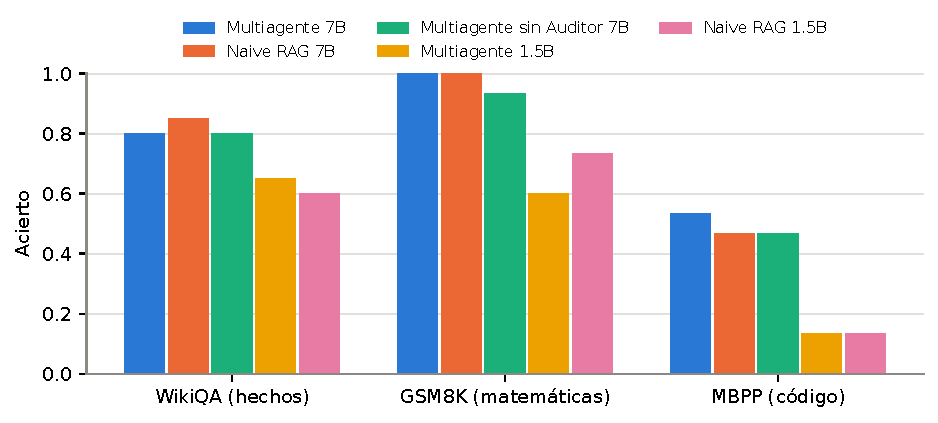
\includegraphics[width=\columnwidth]{fig3_acierto_por_tarea.pdf}
\caption{Acierto por tarea. La ventaja de cada diseño depende de si la tarea permite verificar algo concreto.}
\label{fig:tareas}
\end{figure}

\textbf{Consultas multisalto} (Tabla~\ref{tab:multisalto}). Para medir el caso que motiva la arquitectura se construyeron 15 preguntas que piden los años transcurridos entre dos eventos descritos en dos documentos distintos de WikiQA, con el año verificado en el texto. Todos los errores del Naive RAG ocurren cuando su única recuperación no trae ambos documentos: pide los datos que faltan o inventa un año. El multiagente busca cada evento por separado, resta con Python y casi duplica el acierto; la versión sin Auditor logra lo mismo en menos tiempo, así que aquí la ganancia viene de la descomposición y las herramientas.

\begin{table}[t]
\centering
\caption{Consultas multisalto (dos documentos y una resta).}
\label{tab:multisalto}
\footnotesize
\setlength{\tabcolsep}{3pt}
\begin{tabular}{lcccc}
\toprule
Sistema & Acierto & Ambos docs & Seg. & Llam. \\
\midrule
Multiagente 7B & \textbf{0.93} & 0.80 & 26.3 & 8.7 \\
Naive RAG 7B & \textbf{0.53} & 0.27 & 2.4 & 1.0 \\
Multiagente sin Auditor 7B & \textbf{0.93} & 0.80 & 19.9 & 5.7 \\
\bottomrule

\end{tabular}
\end{table}

\textbf{Auditor accionable.} En una primera versión el Auditor rechazaba el código sin tests con un motivo genérico y el Investigador repetía el mismo reporte; no mejoraba frente a no tener Auditor y duplicaba el tiempo. Al devolver el assert que falla, los tests aprobados suben y la latencia baja (Tabla~\ref{tab:auditor} del Anexo). Un guardrail necesita decir qué corregir, no solo rechazar.

\textbf{Tamaño del orquestador.} Con 1.5B el multiagente es peor que su propio Naive RAG: ignora la regla de usar primero la base local, inventa datos (por ejemplo un sitio web inexistente) y su Auditor los aprueba, lo que se refleja en la Faithfulness más baja de todos los sistemas.

\begin{figure}[t]
\centering
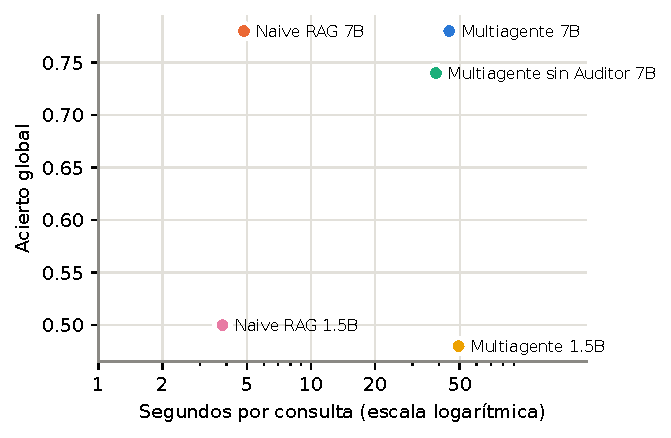
\includegraphics[width=0.92\columnwidth]{fig4_calidad_vs_latencia.pdf}
\caption{Calidad frente a latencia. Los multiagente cuestan cerca de un orden de magnitud más tiempo; reducir el modelo no abarata la arquitectura sin perder calidad.}
\label{fig:latencia}
\end{figure}

\textbf{Costo} (Figura~\ref{fig:latencia}). El grafo cuesta cerca de diez veces la latencia del Naive RAG y el Investigador consume casi todo ese tiempo; el Auditor y el Redactor son baratos (Anexo).

%=====================================================================
\section{Discusión y conclusiones}
%=====================================================================
\begin{enumerate}
\item El multiagente supera al Naive RAG cuando la consulta es compuesta (multisalto) o verificable (código); en preguntas de una sola recuperación empatan y el paso único es más barato y algo más fiel.
\item El Auditor aporta cuando puede comprobar algo objetivo y su retroalimentación es accionable; en código su veredicto predice el resultado en 15 de 15 casos, aunque no siempre logre corregirlo.
\item El tamaño del orquestador pesa más que el número de agentes.
\item Para producción conviene enrutar: Naive RAG por defecto y el grafo completo cuando la consulta pide varios documentos, cálculo o código. La aplicación web del proyecto expone ambos modos con el grafo animado en D3.
\end{enumerate}
\textbf{Limitaciones.} Muestras pequeñas (50 y 15 consultas), con las que solo dos efectos resultan significativos; un solo juez y referencias de WikiQA que a veces difieren de la web actual (el costo del Yankee Stadium). La evaluación necesitó su propia auditoría: el juez inicial generaba preguntas en otro idioma, truncaba la evidencia y extraía afirmaciones del contexto, y el extractor numérico confundía citas con respuestas; todo quedó corregido y registrado.


\small
\begin{thebibliography}{9}
\setlength{\itemsep}{0pt}
\bibitem{yao2023react} S. Yao et al. ReAct: Synergizing reasoning and acting in language models. ICLR, 2023.
\bibitem{yang2015wikiqa} Y. Yang, W. Yih y C. Meek. WikiQA: A challenge dataset for open domain question answering. EMNLP, 2015.
\bibitem{cobbe2021gsm8k} K. Cobbe et al. Training verifiers to solve math word problems. arXiv:2110.14168, 2021.
\bibitem{austin2021mbpp} J. Austin et al. Program synthesis with large language models. arXiv:2108.07732, 2021.
\bibitem{es2023ragas} S. Es et al. RAGAS: Automated evaluation of retrieval augmented generation. arXiv:2309.15217, 2023.
\bibitem{dettmers2023qlora} T. Dettmers et al. QLoRA: Efficient finetuning of quantized LLMs. NeurIPS, 2023.
\bibitem{qwen2025} Qwen Team. Qwen2.5 technical report. arXiv:2412.15115, 2025.
\bibitem{abdin2024phi4} M. Abdin et al. Phi 4 technical report. arXiv:2412.08905, 2024.
\bibitem{reimers2019sbert} N. Reimers e I. Gurevych. Sentence BERT. EMNLP, 2019.
\end{thebibliography}

\clearpage
\onecolumn
\appendix
\section{Anexo}
\label{sec:anexo}

\begin{table}[h]
\centering
\caption{MBPP con el Auditor que rechaza sin devolver el error (v1), con el que devuelve el assert que falla (v2) y sin Auditor.}
\label{tab:auditor}
\begin{tabular}{llccc}
\toprule
Modelo & Versión & Tests MBPP & Rechazos promedio & Segundos \\
\midrule
7B & Sin Auditor & 0.47 & 0.00 & 35.0 \\
7B & Auditor v1 & 0.47 & 1.93 & 82.1 \\
7B & Auditor v2 & 0.53 & 1.00 & 52.9 \\
1.5B & Auditor v1 & 0.13 & 1.60 & 74.6 \\
1.5B & Auditor v2 & 0.13 & 1.53 & 72.1 \\
\bottomrule

\end{tabular}
\end{table}

\begin{figure}[h]
\centering
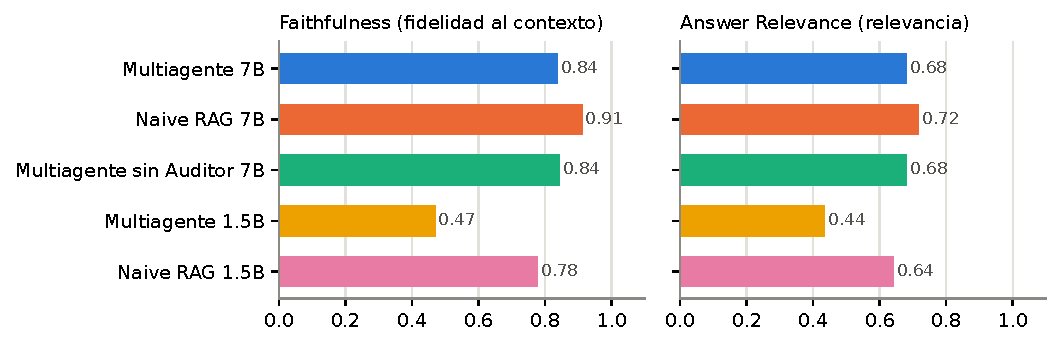
\includegraphics[width=0.75\textwidth]{fig2_ragas.pdf}
\caption{Faithfulness y Answer Relevance por sistema. Con 7B ambos diseños quedan cerca; el multiagente de 1.5B es el que más inventa.}
\end{figure}

\begin{figure}[h]
\centering
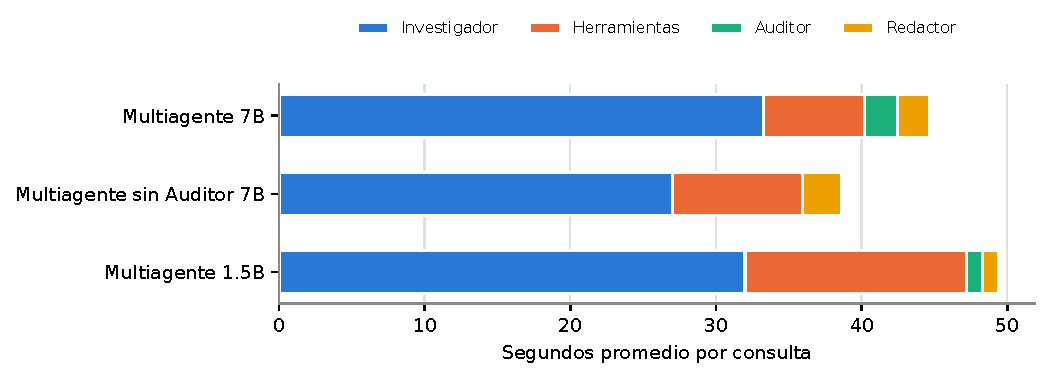
\includegraphics[width=0.48\textwidth]{fig5_latencia_por_agente.pdf}\hfill
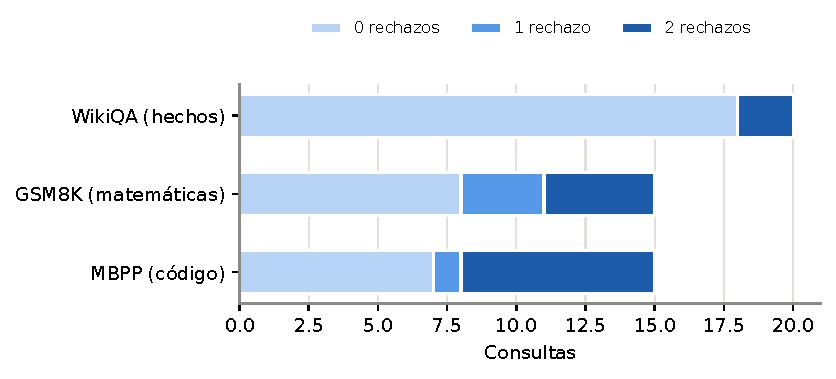
\includegraphics[width=0.48\textwidth]{fig6_rechazos_auditor.pdf}
\caption{Izquierda: el Investigador consume casi todo el tiempo del grafo. Derecha: los rechazos del Auditor se concentran en código y matemáticas, donde puede verificar algo concreto.}
\end{figure}

\begin{figure}[h]
\centering
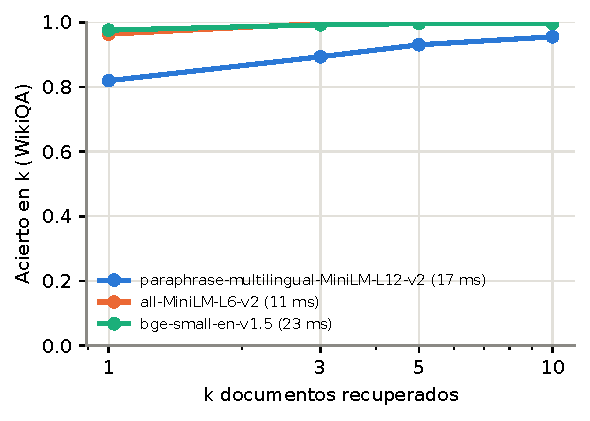
\includegraphics[width=0.5\textwidth]{fig7_recuperacion.pdf}
\caption{Acierto en k del documento correcto de WikiQA. Los modelos en inglés superan al multilingüe del laboratorio y all MiniLM L6 lo hace con la mitad de latencia que bge.}
\end{figure}

\begin{figure}[h]
\centering
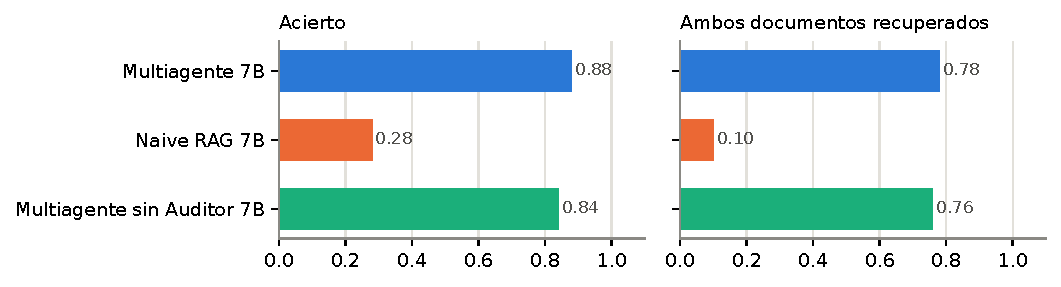
\includegraphics[width=0.8\textwidth]{fig8_multisalto.pdf}
\caption{Consultas multisalto: el Naive RAG solo acierta cuando su única recuperación trae ambos documentos.}
\end{figure}

\end{document}
